\chapter[\hspace{0pt}模型建立与求解]{{\heiti\zihao{3}\hspace{0pt}模型建立与求解}}\label{chapter4: 模型建立与求解}
% \setcounter{page}{4} % 这里要在论文摘要和符号表写完后手动修改页码

\removelofgap
\removelotgap

%% 文章标题架构
% 一级 chapter      : \chapter[\hspace{0pt}模型建立与求解]{{\heiti\zihao{3}\hspace{0pt}模型建立与求解}}\label{chapter4: 模型建立与求解}
% 二级 section      : \section[\hspace{-2pt}问题1:路旅游方案设计]{{\heiti\zihao{-3} \hspace{-8pt}问题1:路旅游方案设计}}\label{section3: 问题1:路旅游方案设计}
% 三级 subsection   : \subsection[\hspace{-2pt}模型建立与求解]{{\heiti\zihao{4} \hspace{-8pt}模型建立与求解}}\label{section3: 模型建立与求解}
% 四级(顶格)        : \noindent\textbf{(1)参数编码与搜索空间}
% 四级(不顶格)      : \textbf{}
% 五级(尽量别用)    : \circled{1} \textbf{$\Delta E_{00}$损失值统计}
% 
%% 公式、图片、表格

% 公式:
% 1. 中间不必加上$$符号
% 2. 在equation后面加上*可以不要自动编号
% \begin{equation}
% \begin{aligned}
%   &u_{i,j}=
%   \begin{cases}
%     v_{i,j}^{(t)},&\text{if } \mathrm{rand}_j\le CR\text{ or } j=j_{rand},\\
%     x_{i,j}^{(t)},&\text{otherwise},
%   \end{cases}
% \end{aligned}
% \end{equation}

% 图片:
% \begin{figure}[h]
% \centering
% \captionsetup{font={small, stretch=1.312}}
% 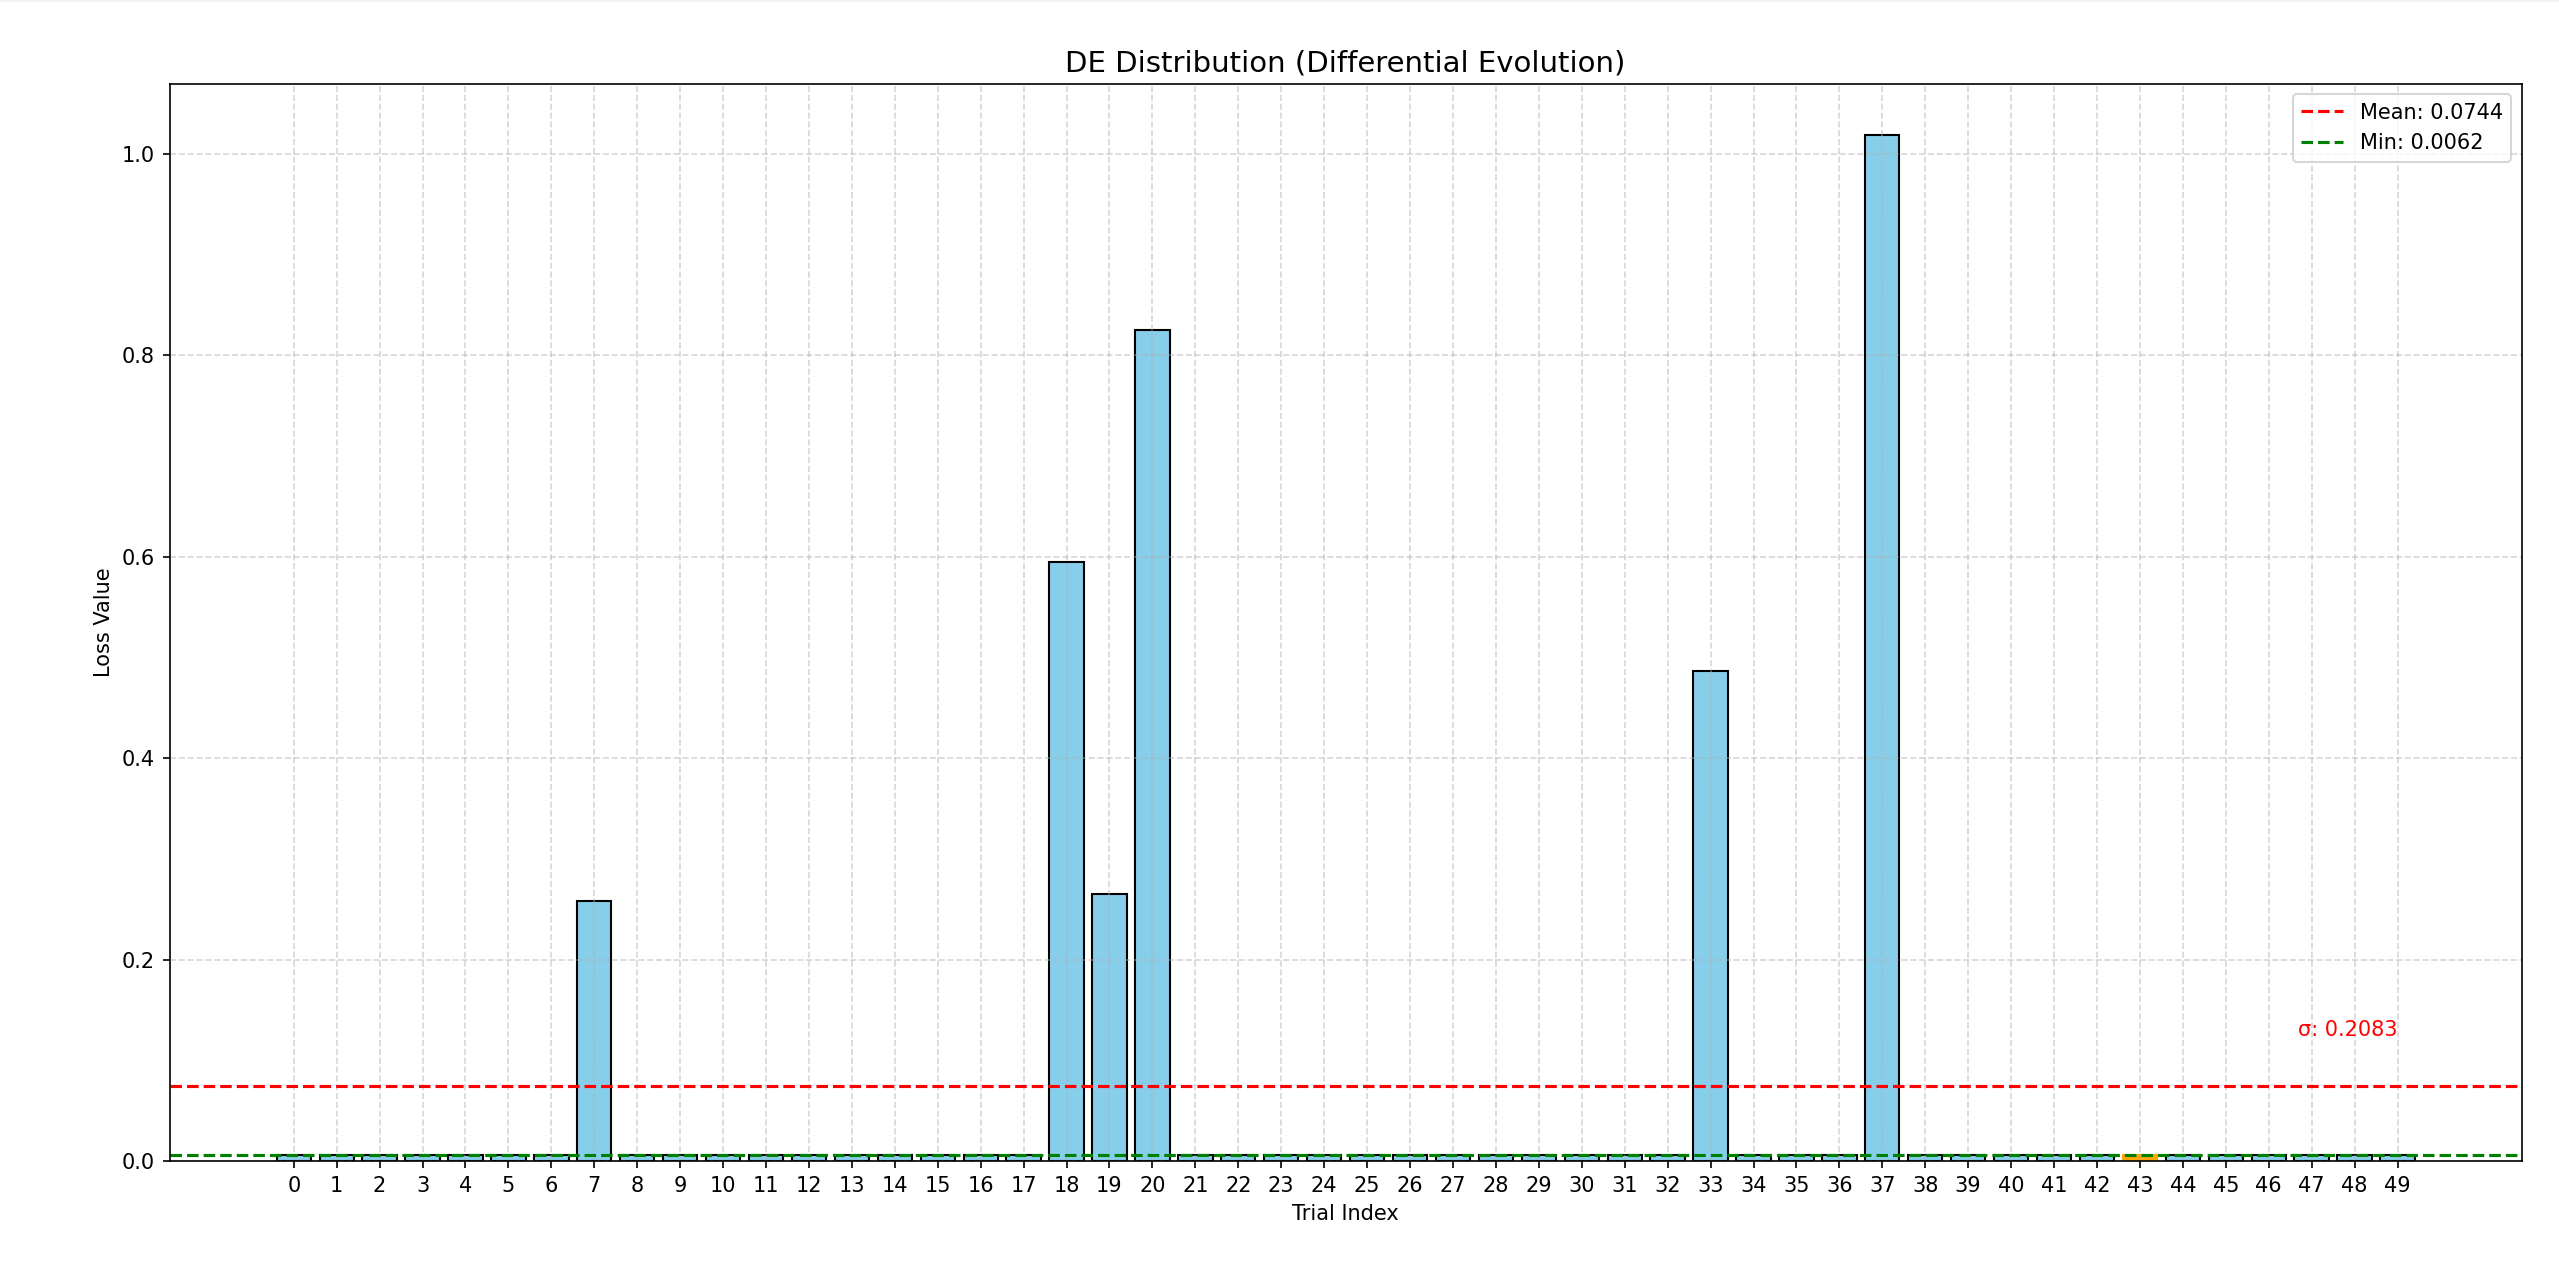
\includegraphics[width=1.0\columnwidth]{figures/DE2000.png}
% \bicaption[50次独立优化实验柱状损失图]{50次独立优化实验柱状损失图。}[Histogram of loss values from 50 independent optimization experiments]{Histogram of loss values from 50 independent optimization experiments.}
% \label{figure3: 柱状loss}
% \end{figure}
% 引用方式:在文字后面加上:\ref{figure3: 柱状loss}

% 表格:
% \begin{table}[h!]
% \small    % 设置表格字体为5号
% \setstretch{1.245}        % 设置具有指定弹力的橡皮长度(原行宽的1.2倍)
% \captionsetup{font={small, stretch=1.512}}
% \centering
%\bicaption[不同基色图像的伽马参数估计结果]{不同基色图像的伽马参数估计结果。}[Gamma parameter estimation results for different primary color images]{Gamma parameter estimation results for different primary color images.}    % 中英文标题


\section[\hspace{-2pt}问题一:农作物种植优化方案设计]{{\heiti\zihao{-3} \hspace{-8pt}问题一:农作物种植优化方案设计}}\label{section3: 问题1:农作物种植优化方案设计}

\subsection[\hspace{-2pt}模型建立与求解]{{\heiti\zihao{4} \hspace{-8pt}模型建立与求解}}\label{section3: 模型建立与求解}

对于此问题,我们首先需要通过设定合理的决策变量,来确定每个地块在每个年份和季节种植的作物面积。每个地块的种植方案需考虑土壤轮作、作物间的轮换以及豆类作物的种植要求。我们还需要加入作物销售限制、耕地面积限制等约束条件,以确保种植计划合理、可行。根据这些条件,我们建立了以下的数学模型:

\textbf{目标函数:}  
为了最大化农业经济效益,我们的目标函数是将所有作物的总收益最大化。作物的收益由其亩产量、市场价格和种植面积决定,同时减去种植成本。公式如下:

\begin{equation}
  \text{Maximize}\quad Z = \sum_{t=2024}^{2030} \sum_{m=1}^{41} \sum_{i=1}^{34} \sum_{s=1}^{2} \left( P_{m,s} \cdot Y_{m,s} \cdot x_{i,m,t,s} - C_{m,s} \cdot x_{i,m,t,s} \right)
\end{equation}

其中,$P_{m,s}$为第 $m$ 类作物在季节 $s$ 的单价;$Y_{m,s}$为第 $m$ 类作物在季节 $s$ 的亩产量;$C_{m,s}$为第 $m$ 类作物在季节 $s$ 的种植成本;$x_{i,m,t,s}$为第 $i$ 块地在第 $t$ 年第 $s$ 季节种植第 $m$ 类作物的面积。

\textbf{豆类作物种植面积要求:}  
根据题目要求,乡村露天地块每年必须种植至少401亩豆类作物,大棚需要种植至少4亩豆类作物。我们定义豆类作物集合 $V_b$,并添加以下约束:

\begin{equation}
\sum_{m \in V_b} \sum_{i=1}^{34} x_{i,m,t} = \frac{1}{3} \cdot 1201 \quad \forall t
\end{equation}

\begin{equation}
\sum_{m \in V_b} \sum_{j=1}^{16} x_{j,m,t} + \sum_{m \in V_b} \sum_{k=1}^{4} x_{k,m,t} = 4 \quad \forall t
\end{equation}

\textbf{作物轮作约束:}  
同一块地不能连续重茬种植相同作物。为此,引入二元变量 $z_{i,m,t}$,当第 $i$ 块地在第 $t$ 年种植第 $m$ 类作物时,$z_{i,m,t} = 1$,否则 $z_{i,m,t} = 0$。因此,约束条件为:

\begin{equation}
z_{i,m,t} + z_{i,m,t+1} \leq 1 \quad \forall i, \forall m, \forall t
\end{equation}

\textbf{耕地面积限制:}  
每年各地块的种植总面积不能超过其可用面积。设 $A_{f_{all}}$ 为第 $i$ 块地的最大种植面积,约束条件为:

\begin{equation}
\sum_{m=1}^{41} x_{i,m,t} \leq A_{f_{all}} \quad \forall i, \forall t
\end{equation}

\textbf{作业便利性约束:}  
每块地的作物种植数有最大数量限制,即每个地块种植的作物种类数量不能超过 $N_{\text{max}}$。公式为:

\begin{equation}
\sum_{m=1}^{41} z_{i,m,t} \leq N_{\text{max}} \quad \forall i, \forall t
\end{equation}

\textbf{求解过程}

\textbf{输入数据:}  
\begin{itemize}
    \item 作物的预期销售量 $D_{m,s}$。
    \item 每种作物的单价 $P_{m,s}$,亩产量 $Y_{m,s}$,种植成本 $C_{m,s}$。
    \item 各地块的可用面积 $A_{f_{all}}$,以及每块地的作物最小种植面积限制 $\delta$。
\end{itemize}

\textbf{模型求解方法:}  
采用混合整数线性规划(MILP)方法求解此优化问题。具体步骤如下:

\begin{itemize}
    \item 使用求解器(如 CPLEX 或 Gurobi)解决模型中的线性约束和目标函数。
    \item 对于每个年度 $t$,按照最大化收益的目标,计算每个地块的作物种植面积分配。
    \item 考虑作物的销售限制、作物轮作约束以及豆类作物种植面积要求,确保在求解过程中遵循所有约束。
\end{itemize}

\textbf{结果输出:}  


\section[\hspace{-2pt}问题二:农作物种植优化方案设计]{{\heiti\zihao{-3} \hspace{-8pt}问题二:农作物种植优化方案设计}}\label{section3: 问题2:农作物种植优化方案设计}

\subsection[\hspace{-2pt}模型建立与求解]{{\heiti\zihao{4} \hspace{-8pt}模型建立与求解}}\label{section3: 模型建立与求解}

对于此问题,我们首先需要通过设定合理的决策变量,来确定每个地块在每个年份和季节种植的作物面积。每个地块的种植方案需考虑作物的销售限制、亩产量、种植成本、销售价格的变化,并考虑气候等不确定因素的影响。我们还需要加入作物销售限制、耕地面积限制等约束条件,以确保种植计划合理、可行。根据这些条件,我们建立了以下的数学模型:

\textbf{目标函数:}  
为了最大化农业经济效益,我们的目标函数是将所有作物的总收益最大化。作物的收益由其亩产量、市场价格和种植面积决定,同时减去种植成本。公式如下:

\begin{equation}
  \text{Maximize}\quad Z = \sum_{t=2024}^{2030} \sum_{m=1}^{41} \sum_{i=1}^{34} \sum_{s=1}^{2} \left( P_{m,s} \cdot Y_{m,s} \cdot x_{i,m,t,s} - C_{m,s} \cdot x_{i,m,t,s} \right)
\end{equation}

其中,$P_{m,s}$为第 $m$ 类作物在季节 $s$ 的单价;$Y_{m,s}$为第 $m$ 类作物在季节 $s$ 的亩产量;$C_{m,s}$为第 $m$ 类作物在季节 $s$ 的种植成本;$x_{i,m,t,s}$为第 $i$ 块地在第 $t$ 年第 $s$ 季节种植第 $m$ 类作物的面积。

\textbf{随机因素:}  
为考虑市场、气候等不确定性因素的影响,我们引入随机符号以模拟作物的销售量、亩产量、种植成本和价格的波动。随机增量符号定义如下:

\begin{itemize}
    \item $\delta^{D}_{m,t}$:需求(销量)变化,遵循 $\mathcal{U}(0.05, 0.10)$ 对于小麦和玉米,其他作物为 $\mathcal{U}(-0.05, 0.05)$;
    \item $\delta^{Y}_{m,t}$:亩产量变化,遵循 $\mathcal{U}(-0.10, 0.10)$;
    \item $\delta^{C}_{m,t}$:成本变化,遵循 $\mathcal{U}(-0.02, 0.02)$;
    \item $\delta^{P}_{m,t}$:单价变化,粮食类为 $\mathcal{U}(-0.02, 0.02)$,蔬菜类作物有5%的正增长,食用菌的单价变化为负,羊肚菌固定每年下降5%。
\end{itemize}

\textbf{需求与收益计算:}  
每个场景下的需求、单产、成本和价格分别由随机增量计算得出,具体为:

\begin{itemize}
    \item $D_{m,t}^{(\omega)}$:第 $\omega$ 场景下的需求;
    \item $Y_{m,t}^{(\omega)}$:第 $\omega$ 场景下的亩产量;
    \item $C_{m,t}^{(\omega)}$:第 $\omega$ 场景下的成本;
    \item $P_{m,t}^{(\omega)}$:第 $\omega$ 场景下的单价。
\end{itemize}

\textbf{约束条件:}  
在优化过程中,我们需要满足以下约束条件:

1. 产量与销量的约束:
作物的产量不应超过需求量,具体为:
\begin{equation}
Y_{m,t}^{(\omega)}\sum_{i}x_{i,m,t,s} \leq D_{m,t}^{(\omega)} \quad \forall m,t,s,\;\forall \omega \in \Omega
\end{equation}

2. 耕地面积约束:
每块地的种植总面积不能超过其可用面积,设第 $i$ 块地的最大可用面积为 $A_{f_{all}}$,约束条件为:
\begin{equation}
\sum_{m=1}^{41} x_{i,m,t} \leq A_{f_{all}} \quad \forall i, \forall t
\end{equation}

3. 作物种植数量限制: 
每块地的种植作物数量有最大数量限制,具体为:
\begin{equation}
\sum_{m=1}^{41} z_{i,m,t} \leq N_{\text{max}} \quad \forall i, \forall t
\end{equation}

\textbf{求解过程}

\textbf{输入数据:}  
\begin{itemize}
    \item 作物的预期销售量 $D_{m,s}$;
    \item 每种作物的单价 $P_{m,s}$,亩产量 $Y_{m,s}$,种植成本 $C_{m,s}$;
    \item 各地块的可用面积 $A_{f_{all}}$,以及每块地的作物最小种植面积限制 $\delta$。
\end{itemize}

\textbf{模型求解方法:}  
采用蒙特卡洛采样法(SAA)与混合整数线性规划(MILP)方法求解此优化问题。具体步骤如下:

\begin{itemize}
    \item 使用求解器(如 Gurobi 或 CPLEX)解决模型中的线性约束和目标函数。
    \item 对于每个年度 $t$,按照最大化收益的目标,计算每个地块的作物种植面积分配。
    \item 考虑作物的销售限制、作物轮作约束以及豆类作物种植面积要求,确保在求解过程中遵循所有约束。
\end{itemize}

\textbf{结果输出:}  
求解器返回最优的种植方案,输出每个地块在每年各季节的种植作物和面积。该结果可以填入对应的模板文件中。

通过此优化模型和求解过程,我们可以得到2024至2030年间的最优种植方案,确保农作物种植的经济效益最大化,同时满足所有农业生产和管理要求。

\subsection[\hspace{-2pt}算法伪代码流程]{{\heiti\zihao{4} \hspace{-8pt}算法伪代码流程}}\label{section3: 算法伪代码流程}

以下为模型求解的伪代码流程:

\begin{algorithm}[H]\small
\setstretch{1.245} % 设置行距
\renewcommand{\algorithmcfname}{算法}
\caption{农作物种植优化模型求解伪代码流程}
\KwIn{作物的预期销售量 $D_{m,s}$、单价 $P_{m,s}$、亩产量 $Y_{m,s}$、种植成本 $C_{m,s}$、可用面积 $A_{f_{all}}$、最小种植面积 $\delta$}
\KwData{场景数 $S$,风险系数 $\lambda$}

\textbf{步骤1:场景数据生成}\\
\For{$\omega = 1$ \textbf{to} $S$}{
    生成随机增量 $\delta^{D}_{m,t}$、$\delta^{Y}_{m,t}$、$\delta^{C}_{m,t}$、$\delta^{P}_{m,t}$\\
    计算派生参数 $D_{m,t}^{(\omega)}$、$Y_{m,t}^{(\omega)}$、$C_{m,t}^{(\omega)}$、$P_{m,t}^{(\omega)}$\\
}

\textbf{步骤2:逐年逐地块优化}\\
\For{$t = 2024$ \textbf{to} $2030$}{
    \For{$i = 1$ \textbf{to} $34$}{
        计算各作物种植面积 $x_{i,m,t,s}$ 以最大化收益\\
        计算并更新作物种植成本与销售收益\\
        验证各项约束条件(如面积限制、轮作约束等)\\
    }
}

\textbf{步骤3:求解优化模型}\\
求解并获得最优解 $x^\star$\\

\textbf{步骤4:输出结果}\\
输出每年各地块的作物种植方案\\

\label{algorithm:crop_optimization}
\end{algorithm}







\section[\hspace{-2pt}问题三:农作物种植优化策略(考虑价格弹性、替代性与互补性)]{{\heiti\zihao{-3} \hspace{-8pt}问题三:农作物种植优化策略(考虑价格弹性、替代性与互补性)}}\label{section3: 问题3:农作物种植优化策略}

\subsection[\hspace{-2pt}模型建立与求解]{{\heiti\zihao{4} \hspace{-8pt}模型建立与求解}}\label{section3: 模型建立与求解}

在第三问中,我们需要基于第二问的模型,加入考虑农作物间的价格弹性、替代性和互补性等因素,来设计2024~2030年间的最优种植策略。根据实际市场情况,作物的价格、销量、种植成本之间存在相互影响,尤其是作物间的替代性和互补性需要特别考虑。本模型的目标是最大化农作物种植的经济效益,同时考虑供需关系对价格和销量的影响。

\textbf{目标函数:}  
与第二问相似,我们的目标函数依然是最大化农作物的收益,但是这次需要对价格和销量进行调整。通过引入价格和需求弹性系数,将作物的价格和需求纳入优化目标。具体公式如下:

\begin{equation}
  \text{Maximize}\quad Z = \sum_{t=2024}^{2030} \sum_{m=1}^{41} \sum_{i=1}^{34} \sum_{s=1}^{2} \left( \tilde{P}_{m,t} \cdot Y_{m,t}^{\text{eff}} \cdot x_{i,m,t,s} - C_{m,t} \cdot x_{i,m,t,s} \right)
\end{equation}

其中,$\tilde{P}_{m,t}$为考虑替代性和互补性后的调整价格,$Y_{m,t}^{\text{eff}}$为考虑轮作增益后的有效亩产量,$x_{i,m,t,s}$为第 $i$ 块地在第 $t$ 年第 $s$ 季节种植第 $m$ 类作物的面积。

\textbf{有效需求:}  
在此模型中,我们将有效需求($\tilde{D}_{m,t}$)替代原始的需求量($D_{m,t}$),以便反映作物价格与销量之间的关系。有效需求是通过价格弹性和市场供需关系进行调节的,公式如下:

\begin{equation}
  \tilde{D}_{m,t} = D_{m,t} \left( 1 + \eta_{m} \cdot \frac{\tilde{P}_{m,t} - P_{m,t}}{P_{m,t}} \right)
\end{equation}

\textbf{作物替代性与互补性:}  
我们引入了替代性系数和互补性系数来调整作物之间的供需关系。作物的需求会受到同类作物增加(替代性)或互补作物增加(互补性)的影响。替代性和互补性会影响作物的价格和需求,公式如下:

\begin{equation}
  \tilde{P}_{m,t} = P_{m,t} \left( 1 - \sum_{k \in \text{Subs}(m)} \alpha_{k \to m} \frac{Q_{k,t}}{Q_{k}^{\star}} + \sum_{k \in \text{Comp}(m)} \eta_{k \to m} \frac{Q_{k,t}}{Q_{k}^{\star}} \right)
\end{equation}

\begin{equation}
  \tilde{D}_{m,t} = \tilde{D}_{m,t} - \sum_{k \in \text{Subs}(m)} \alpha_{k \to m} Q_{k,t} + \sum_{k \in \text{Comp}(m)} \eta_{k \to m} Q_{k,t}
\end{equation}

\textbf{轮作增益:}  
为了简化模型,我们假设轮作能够增加单产(例如,豆类与玉米的轮作可增加10%的单产)。在模型中,我们将轮作增益系数($\theta^{\text{rotation}}_m$)加入到作物的单产中,来考虑轮作的正向影响。具体形式如下:

\begin{equation}
  Y_{i,m,t}^{\text{eff}} = Y_{m,t} \cdot \left( 1 + \theta^{\text{rotation}}_m \cdot z_{i,m,t-1} \right)
\end{equation}

其中,$z_{i,m,t}$为二元变量,表示第 $i$ 块地在第 $t$ 年是否种植第 $m$ 类作物。

\subsection[\hspace{-2pt}求解过程]{{\heiti\zihao{4} \hspace{-8pt}求解过程}}\label{section3: 求解过程}

\textbf{输入数据:}  
\begin{itemize}
  \item 作物的预期销售量 $D_{m,t}$。
  \item 每种作物的单价 $P_{m,t}$,亩产量 $Y_{m,t}$,种植成本 $C_{m,t}$。
  \item 作物替代性系数 $\alpha_{k \to j}$ 和互补性系数 $\beta_{k \to j}$。
  \item 各地块的可用面积 $A_{f_{all}}$,以及每块地的作物最小种植面积限制 $\delta$。
  \item 每种作物的轮作增益系数 $\theta^{\text{rotation}}_m$。
\end{itemize}

\textbf{模型求解方法:}  
我们采用混合整数线性规划(MILP)方法来求解该问题,具体步骤如下:

\begin{itemize}
  \item 对于每个年度 $t$,利用供给和价格弹性关系,计算调整后的价格 $\tilde{P}_{m,t}$ 和有效需求 $\tilde{D}_{m,t}$。
  \item 引入替代性和互补性调整项,根据作物间的相互关系调整作物的市场需求。
  \item 考虑轮作增益,计算每个地块的有效单产 $Y_{m,t}^{\text{eff}}$。
  \item 使用求解器(如 Gurobi 或 CPLEX)求解优化问题,得到每个地块的最优种植面积和作物分配方案。
\end{itemize}

\textbf{结果输出:}  
求解器返回最优的种植方案,输出每个地块在每年各季节的种植作物和面积,并提供每种作物的调整后价格和有效需求。通过分析这些结果,可以得出最优的农作物种植策略,以最大化2024至2030年间的经济效益。

通过该优化模型,我们能够考虑作物间的价格弹性、替代性与互补性以及轮作效应,从而得到更加精细化和可行的农作物种植策略,进一步提升农业生产的效益并减少市场风险。


\subsection[\hspace{-2pt}结果分析]{{\heiti\zihao{4}\hspace{-8pt}结果分析}}\label{subsec:3-model-build}



